% !TEX root = ../main.tex
%-------------------------------------------------------------------------------
%-------------------------------------------------------------------------------
\begin{frame}\frametitle{In a nutshell}
\hspace{1.5cm}
\begin{quote}\Large
	We provide a platform for economists, mathematicians, and computational scientists to facilitate the transdisciplinary collaboration in the development, analysis, and application of computational economic models. Together, we expand the set of possible economic questions that we can address and improve the quality of our	answers.
\end{quote}


\end{frame}
%-------------------------------------------------------------------------------
%-------------------------------------------------------------------------------
\begin{frame}\frametitle{Computational modeling in economics}

	\begin{multicols}{2}
	\heading{Motivation}\vspace{0.3cm}
	\begin{itemize}\setlength\itemsep{1em}
	\item Facilitate learning
	\item Study mechanisms
	\item Predict public policies
	\end{itemize}

	\pause

  \heading{Transdisciplinary in nature}\vspace{0.3cm}
	\begin{itemize}\setlength\itemsep{1em}
	\item Economic model
	\item Mathematical framework
	\item Computational implementation
	\end{itemize}
	\end{multicols}

\end{frame}

%-------------------------------------------------------------------------------
%-------------------------------------------------------------------------------
\begin{frame}\frametitle{New tooling for an old idea}

THE greatest improvement in the productive powers of labor, and the greater part of the skill, dexterity, and judgment with which it is anywhere directed, or applied, seem to have been the effects of the division of labor.


Adam Smith
\textbf{maybe a black-white picutre of Adam Smith on the left , or bottom, wherever nice ...}

\end{frame}

%-------------------------------------------------------------------------------
%-------------------------------------------------------------------------------
\begin{frame}\frametitle{Partners}\vspace{1.0cm}

\begin{columns}[t]
	\column{.5\textwidth}
	\centering \\
  % Institute for Numerical Simulation
  
\includegraphics[width=0.3\textwidth]{material/crop-cooperation-ins.png} \\\vspace{-0.5cm}
  \footnotesize{Institute for \\ Numerical Simulation}\vspace{0.3cm}



  % HEC Lausanne
	\column{.5\textwidth}
	\centering
	
\includegraphics[width=0.45\textwidth]{material/crop-cooperation-diw.png}\\
	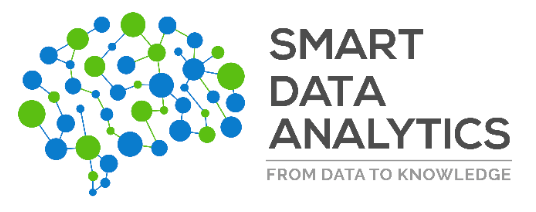
\includegraphics[width=0.45\textwidth]{material/crop-cooperation-sda.png}\\

	
\includegraphics[width=0.45\textwidth]{material/crop-cooperation-ssb.png}\\

	% Statistics Norway
	% Institute for Numerical Simulation
  
\includegraphics[width=0.45\textwidth]{material/crop-cooperation-limes.png}\\
	\vspace{1.75cm}
  
\includegraphics[width=0.45\textwidth]{material/crop-cooperation-lausanne.png} \\

  \column{.5\textwidth}
  \centering \\

\end{columns}

\end{frame}
%-------------------------------------------------------------------------------
%-------------------------------------------------------------------------------
\begin{frame}\frametitle{What we are doing}

\alert{Economic models}

\begin{itemize}\setlength\itemsep{1em}
	\item \makebox[2.25cm][l]{\alert<1>{respy}}
                \only<1>{
                        \explanation{
												Finite-horizon discrete Markov decision problem\\
                                Labor economics
                        }
                }
	\item \makebox[2.25cm][l]{\alert<2>{ruspy}}
                \only<2>{
                        \explanation{
												Infinite-horizon discrete Markov decision problem\\
                                Industrial organization
                        }
                }

		\item \makebox[2.25cm][l]{\alert<3>{pydsge}}
										\only<3>{
														\explanation{
														Dynamic stochastic general equilibrium model\\
														Monetary economics
														}
										}

\end{itemize}

\end{frame}
%-------------------------------------------------------------------------------
%-------------------------------------------------------------------------------
\begin{frame}\frametitle{What we are doing}

	\heading{Analysis pipeline}\vspace{0.3cm}

	\begin{itemize}\setlength\itemsep{1em}
	        \item \makebox[2.25cm][l]{\alert<1>{estimagic}}
	                \only<1>{
	                        \explanation{
													Numerical optimization \\
	                                Estimating structural econometric models
	                        }
	                }
					\item \makebox[2.25cm][l]{\alert<2>{econsa}}
	                \only<2>{
	                        \explanation{%
													Sensitivity analysis \\
																	Assessing uncertainty of model implications
																	                        }
	                }

									\item \makebox[2.25cm][l]{\alert<3>{robupy}}
					                \only<3>{
					                        \explanation{%
																	Robust optimization \\
																					Incorporating model ambiguity
																					                        }
					                }

	\end{itemize}

\end{frame}
%-------------------------------------------------------------------------------
%-------------------------------------------------------------------------------
\begin{frame}\frametitle{Development}

	\begin{multicols}{2}
	\heading{Workflow}\vspace{0.3cm}
	\begin{itemize}\setlength\itemsep{1em}
	\item GitHub organization
	\item Code reviews
	\item Testing harness
	\item Continuous integration
	\end{itemize}

\columnbreak
	\pause

  \heading{Support}\vspace{0.3cm}
	\begin{itemize}\setlength\itemsep{1em}
	\item Documentation
	\item Chatroom
	\item Hackathon
	\item Conferences
	\end{itemize}
	\end{multicols}

\end{frame}
%-------------------------------------------------------------------------------
%-------------------------------------------------------------------------------
